\chapter{Design}
This chapter documents the major design decisions in the process of building a tool that supports the hinting tool concept from \ref{chap:conceptual_design}. It focuses on building models that enable translations from the use case representations to tests -- focusing on broad test coverage.\\\\
We introduce the term of ``system state'', which refers to the state system under development. This state is covered in more detail in section \ref{ssec:system-state}

\section{Meta model}
\begin{figure}[!htbp]
  \centering
  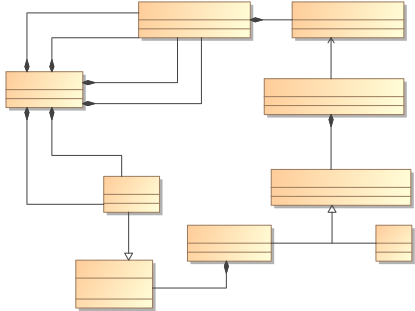
\includegraphics[scale=0.9]{img/3rd_iteration_meta_model}
  \caption{Meta model of the third concept}
  \label{fig:3rd_iteration_meta_model}
\end{figure}
\noindent This section discusses an evolved and simplified version of the meta model introduced in chapter \ref{chap:conceptual_design}, and covers the changes that happened when the model transitioned from concept to design.\\\\
A central concept that was removed, is the actor actions. While they provided additional information about what actors were capable of, they added little or no value to tests. The predicates that signified the pre- and postcondition have been turned into simple use blocks, which effectively means that the mapper needs to explicitly break the execution within the conditional steps, in the case of an unmet condition.\\\\
When performing a translation, every use case step will be broken down into a set of decomposed steps. A decomposed step is an \emph{ordered} list of either a definition or just a text. The decomposition is a reversible process, that will be performed by the use of a definition set. A definition set is the information which added by the use case writer and links domain concepts to use cases. Definitions are used to infer which concepts or actors need to passed to the generated test case functions.

\section{Translating a use case}
Once we have built the use case models, translation of a them is a matter determining which paths they contain and translating them to the test function calls. The signatures of the functions are automatically inferred by the concept types linked in definitions.\\\\
During the design process, three major constraints for use cases -- in regards to test generation -- were defined. 
\begin{description}
  \item[Entries:] Every entry in a use case scenario is a synchronous self-contained action. Single steps may mutate the system state
  \item[Termination:] A use case scenario should always terminate.
  \item[No extensions nesting:] A design decision that simplified the path determination.
\end{description}
We treat the use case scenario with extensions as a directed graph -- potentially containing cycles. Every node of the graph represents a use case step and every edge the invocation of the next step. An example of a use case graph is shown in figure \ref{fig:use-case-graph}. It consists of a main scenario, which are all the $s_n$ states (state $s_1$ to $s_5$) and an exit point. The exit point is provided to signify explicit termination for the main scenario -- but especially for use case extensions that never return to the main scenario, but merely terminate the use case. The extension node $e_{3.1}$ represent an extension that this exact behavior.\\\\
The next subsection goes into more detail on how to extract the different paths from the use case graph.

\begin{figure}[!htbp]
\centering
\begin{tikzpicture}[->,>=stealth',shorten >=0.8pt,auto,node distance=1.8cm,
thick,
extension1 node/.style={circle,fill=blue!20,draw,font=\sffamily\bfseries},
extension2 node/.style={circle,fill=orange!20,draw,font=\sffamily\bfseries},
extension3 node/.style={circle,fill=brown!20,draw,font=\sffamily\bfseries},
exit node/.style={circle,fill=red!20,draw,font=\sffamily\bfseries},
chosen node/.style={circle,fill=green!20,draw,font=\sffamily\bfseries}]

%Scenario
\node[chosen node] (s1) {$s_1$};
\node[chosen node] (s2) [below of=s1] {$s_2$};
\node[chosen node] (s3) [below of=s2] {$s_3$};
\node[chosen node] (s4) [below of=s3] {$s_4$};
\node[chosen node] (s5) [below of=s4] {$s_5$};
\node[exit node] (exit) [below of=s5] {$exit$};

%Extension 1
\node[extension1 node] (e1_1) [left of=s2] {$e_{1.1}$};

%Extension 2
\node[extension2 node] (e2_1) [right of=s4] {$e_{2.1}$};

%Extension 3
\node[extension3 node] (e3_1) [left of=s4] {$e_{3.1}$};

%Paths
\path[every node/.style={font=\sffamily\small}]
(s1)   edge node [] {} (s2)	
(s2)   edge node [] {} (s3)
       edge node [] {} (e1_1)
(s3)   edge node [] {} (s4)
(s4)   edge node [] {} (s5)
       edge node [] {} (e2_1)
       edge node [] {} (e3_1)
(s5)   edge node [] {} (exit)

(e1_1) edge[bend right] node [] {} (s3)
(e2_1) edge[bend right] node [] {} (s2)
(e3_1) edge[bend right] node [] {} (exit)
;
\end{tikzpicture}
\caption{Graph depicting different paths through a use case}
\label{fig:use-case-graph}
\end{figure}
\subsection{Determining paths}
\label{ssec:use-case-paths}
A path of a use case is any graph path that traverses the graph from the initial state $s_1$ to the ($exit$) node. In the use case graph in figure \ref{fig:use-case-graph}, we have the following paths - not counting loops.\\\\
\begin{itemize}
  \item Main scenario
  \item Extension 1
  \item Extension 2
  \item Extension 3
  \item Extension 1 and 2
  \item Extension 1 and 3  
  \item Extension 2 and 1
  \item Extension 2 and 3  
  \item Extension 3 and 3
  \item Extension 1, 2 and 3
  \item Extension 2, 1 and 3
\end{itemize}
\noindent The basic path of an extension (the one that diverts from the main scenario, and goes straight back to it, once finished can be represented as the union of the path leading in, the path of extension scenario, and the path from the exit point of the extension, to the exit point of the use case (\ref{eqn:exten-base-path}). 
\begin{equation}
p_{exten} = \left\lbrace s_1 \dots E_{entry} \right\rbrace \bigcup E_{scenario} \bigcup \left\lbrace E_{entry} \dots exit \right\rbrace
\label{eqn:exten-base-path}
\end{equation}
Harvesting the additional paths will be a matter of combining the scenario of the use ($E_{scenario}$) with the all the different possible entry and exit paths, as seen in the itemized list above. Efficient algorithms for enumerating all simple paths of a graphs already exist\cite{rubin1978enumerating}, and will not be covered in more detail in this thesis.\\\\
Once a list of paths is retrieved, it is possible to convert every path, which is essentially a list of active actions either performed by, or affecting, the primary actor. This list will be translated into a test by converting it into code snibblet, and join them together in a code block that becomes the body of a test function.\\\\
Up until now, the fact that back edges (edges that go backwards in the directed graph) can occur, has been ignored. These edges raises the bar for identifying unique paths, as it introduces loops. Loops are potentially infinite, and needs to be detected and mapped appropriately.\\\\
The loop detection is quite simple if we disallow nested extensions. In that case, the loop detection can be performed solely by detecting that the return point of the extension is not before the entry point in the main scenario. When a loop is detected in an extension, the extension may be flagged as ``looping''.\\\\

\noindent Loops make it impossible to achieve 100\% test coverage, but we could emulate the behavior by defining a fixed number times that the loop must execute, and a fixed path that it should always take during the loops. While this is far from optimal, the test generation tool could provide some convenience functions.The should aid the use case writer in choosing which paths should be taken in which loop execution, and how many time it should loop.

%The basic rules for path collection is;
\section{Mapping the test to the domain}
%TODO mention errors, how to emulate errors. We need to have a use case that describes the exact circumstances under which the error arises.
This section discussed the individual components of a use case with the perspective of converting it into an executable test. In order to write up functions that implement the generated function block stubs in actual system behavior, a programming model is presented in this section.\\\\
The programming model builds upon the constrain of having the use case represented as an list ordered list of steps that are unrolled into paths, that represent the different ways a use case can play out. The steps of these paths need to be executed in order.
\subsection{Step execution}
\label{sec:step-execution}
\label{sec:use-case-environment}
Executing a test of given use case path may be considered a long function call-chain. Each new function call passes its computed state onto the next function. This method of passing along the state is a common pattern is interpreters and compilers, where this state is referred to as ``the environment'', and s initially fed into the tests with a list of variable and function definitions -- similar to those our meta model. In our test-case compiler we adopt this concept. One of the large benefits is to have the ability to have an exit procedure that performs state clean upon exit of every use case.\\\\
An execution of a use case path that consists of $n$ steps could look like the expression in \ref{eqn:path-evaluation}. 
\begin{equation}
Postcondition \rightarrow S_n \rightarrow S_{n-1} \rightarrow \dotsb \rightarrow S_2 \rightarrow S_1 \rightarrow Precondition \rightarrow env
\label{eqn:path-evaluation}
\end{equation}
The expression function is applied to the statement, then the result is applied to the matcher which then returns a success or failure value depending on the outcome of the evaluation. This execution model is very model is very similar to monadic function use in functional programming, where every function carries the state needed by the next function. The model may also be, represented in procedural languages by a list of statements that only operate on input parameters and return their result.

\subsection{Test case environment}
\label{sec:test_case_state}
%TODO the requirements to the state is inferred by the used concepts.

A runnable test consists of three basic steps; setup, run and teardown. Setup and teardown is different from pre- and postcondition in that they are unrelated to the test itself, they merely make sure that objects are initialized with right values and, in general, are in the state that the test expects.

There needs to be an executable domain model programmed, not necessarily complete, but the concepts covered in the use cases should at least be there. So for the use case ``Send message to contact'' (see appendix \ref{appendix:use-cases}). We need at least a class representing the actor ``Receptionist'', and a class representing a message. The actions performed by the actor could then either be class methods, or simply functions taking the primary actor (or more exact; classes of the actor), as an argument.

How do we define which objects are currently in the test harness? In our implementation, we have made a configuration file that, potentially could be auto-generated from a description of which domain types the objects have, what their internal data is, and when they need to be present.

\subsection{Mapping branches}
Use cases may branch out and go to alternatives actions. These branches are associated with errors, and may be difficult to emulate. One possibility is to use an assumption mapping here, and treat the event or decision as having occurred. For active decisions taken by the primary actor, for example an action taken to better serve a customer request, it is easy to assume. Injecting errors in a running system is something else entirely... %TODO Finish.

\subsection{System state}
\label{ssec:system-state}
%TODO relate this to preconditions.
If we assume that the use cases are self-contained\cite{larman2005} in the way that every action and alternative, for a given actor, may be put into a single (large) use case, then it should also be possible to treat use cases as functions that operate on a global system state.\\\\

Use cases may also specify some expectations to the system state. This is what is defined as preconditions. If we, however, maintain a system state analogy, we may model use case executions as a set of mutation functions that affect the global system state.\\\\
A simple example; a actor \emph{accountant} has a use case \emph{accountant creates invoice}. This use case requires that the \emph{accountant} actor has previously been created. The creation could be provided by the \emph{admin} actor's \emph{admin creates accountant} use case.
\begin{figure}[h]
\includegraphics[scale=0.75]{\imgdir system-state-machine-relations}
\centering
\caption{State machine of perceived system state}
\label{fig:system-state-machine-relations}
\end{figure}
So, the \emph{accountant creates invoice} effectively has a precondition that is provided by \emph{admin creates accountant} to make the global state match what is expected to execute the \emph{accountant creates invoice}. The concept is illustrated in figure \ref{fig:system-state-machine-relations} where \emph{Use Case 1} is a prerequisite to \emph{Use Case 2}, but \emph{Use Case 3} has no prerequisites. In order to reach completion (termination) and coverage of \emph{Use Case 2}, \emph{Use Case 1} has to be executed.\\
Each use case state (an example is \textbf{Post-UC1} in figure \ref{fig:system-state-machine-relations}) is a super-state that contains the state space of every alternative scenario. Basically, every node, of every path extracted from the graphs described in section \ref{ssec:use-case-paths} is also a state, and every edge; the mutation function.\\\\
This model is useful to consider when programming the test support tools, and may even be supported by a concept, such as the event stack validation described in appendix \ref{appendix:event-stack-validation}, where the states and transitions are logged, and replayed through a set of state machines. But, for the majority of implementations, it should be considered a programming model. Using this model, developers may also chose to build their precondition mappings as other use cases.



\subsection{Simulating error conditions}
Any use case statement may be mapped to an assumption, an error or an assumption.

\subsection{Detecting logic errors in use cases}

\begin{description}
  \item[Skipping actions may be prohibited:] Should it be possible to jump ahead in the use case?
  \item[Primary actor must participate:] The primary actor is important, as this is the stakeholder that defines the perspective and scope of the test. The primary is the person that starts the use case via an active action, or receives a start signal from another actor -- the system for instance. The primary actor must also be part of the main scenario, and an analysis error should occur if this is not the case.

\end{description}


%TODO there are problems with duplicate words; table table.

%TODO Integrate and finalize notes below.


%\section{Test framework}
% You need to write a test framework containing object pools, factory classes aso.
%\subsection{Exploiting injected semantics}
%How may we benefit from additional semantics? We can identify rubbish postconditions, such as predicates that involve objects that are either not modified in the statements, or simply never referenced.

%\section{Evaluating a use case}
%A use case can be modeled as a function taking in a starting environment and returning a boolean value, so $U \rightarrow env \rightarrow bool$

\subsection{Running the analysis}
Having a set of definitions, we can detect actors and concepts from textually analysing the text of every UseCaseEntry object. The analysis is quite simple, and merely looks for occurrences of the definition by comparing strings.

\subsection{Capabilites of an actor}
If we were to add additional domain knowledge to the use cases, then we would also be able to extract capabilities easily.
%yada yada, use case example: actor does something to some other thing
% it means the the actor can do something to some other thing.

\subsection{Providing initial information}
%How to add receptions, users and other stuff?
%Could this be done with a use case as well?


